\def\mytitle{PARABOLA}
\def\myauthor{SRAVANI VUNNAVA}
\def\contact{sravani21vunnava@gmail.com}
\def\mymodule{Future Wireless Communication (FWC)}
\documentclass[10pt, a4paper]{article}
\usepackage[a4paper,outer=1.5cm,inner=1.5cm,top=1.75cm,bottom=1.5cm]{geometry}
\twocolumn
\usepackage{setspace}
\usepackage{graphicx}
\graphicspath{{./images/}}
\usepackage[colorlinks,linkcolor={black},citecolor={blue!80!black},urlcolor={blue!80!black}]{hyperref}
\usepackage[parfill]{parskip}
\usepackage{lmodern}
\usepackage{tikz}
 \usepackage{physics}
%\documentclass[tikz, border=2mm]{standalone}
\usepackage{karnaugh-map}
\usepackage{tabularx}
\usetikzlibrary{calc}
\usepackage{amsmath}
\usepackage{amssymb}
\renewcommand*\familydefault{\sfdefault}
\usepackage{watermark}
\usepackage{lipsum}
\usepackage{xcolor}
\usepackage{listings}
\usepackage{float}
\usepackage{titlesec}
\providecommand{\mtx}[1]{\mathbf{#1}}
\titlespacing{\subsection}{1pt}{\parskip}{3pt}
\titlespacing{\subsubsection}{0pt}{\parskip}{-\parskip}
\titlespacing{\paragraph}{0pt}{\parskip}{\parskip}
\newcommand{\figuremacro}[5]{//
    \begin{figure}[#1]
        \centering
        \includegraphics[width=#5\columnwidth]{#2}
        \caption[#3]{\textbf{#3}#4}
        \label{fig:#2}
    \end{figure}
}
\providecommand{\brak}[1]{\ensuremath{\left(#1\right)}}
\providecommand{\lbrak}[1]{\ensuremath{\left(#1\right.}}
\providecommand{\rbrak}[1]{\ensuremath{\left.#1\right)}}
\providecommand{\sbrak}[1]{\ensuremath{{}\left[#1\right]}}
\newcommand{\myvec}[1]{\ensuremath{\begin{pmatrix}#1\end{pmatrix}}}
\let\vec\mathbf
\lstset{
frame=single, 
breaklines=true,
columns=fullflexible
}

\title{\mytitle}
\author{\myauthor\hspace{1em}\\\contact\\FWC22040\hspace{6.5em}IITH\hspace{0.5em}\mymodule\hspace{6em}ASSIGN-6}
\date{}
\begin{document}
 \maketitle
 \tableofcontents
 \section{Problem}
If a chord, which is not a tangent, of the parabola $y^2=16x$ has the equation $2x+y=p$, and midpoint $\myvec{h\\k}$, then which of the following is (are) possible value(s) of p,h and k
	\section{Construction}
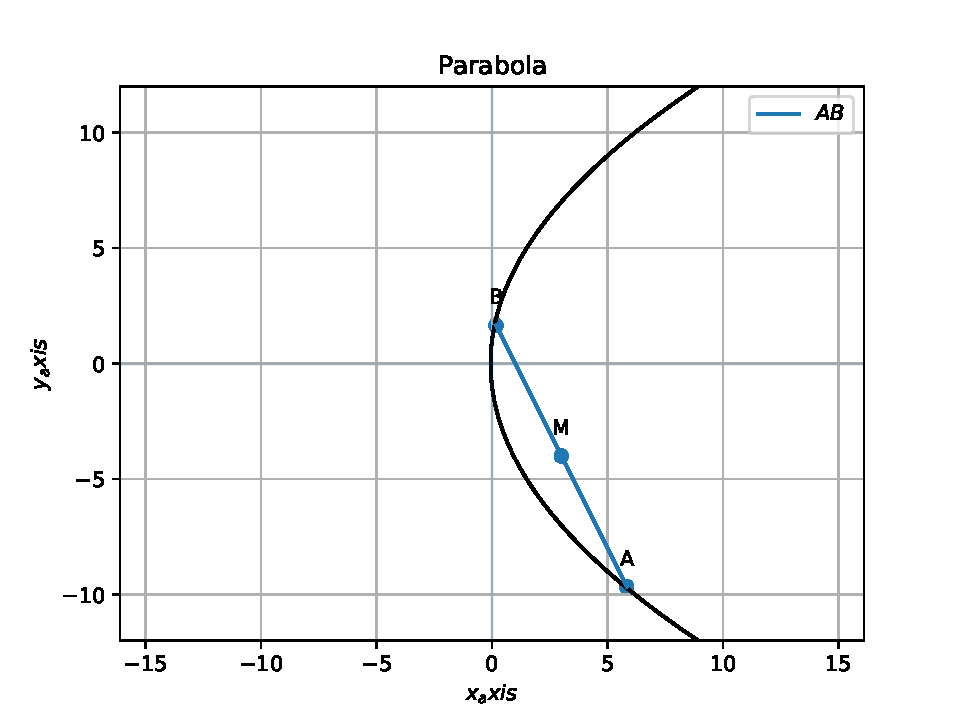
\includegraphics[scale=0.5]{par.pdf}

\section{Solution}
The given equation of line is
\begin{equation}
    x = \myvec{0 \\ p} + \mu\myvec{1\\-2}
\end{equation}
The equation of parabola is:
\begin{equation}
    \vec{X}^T\vec{V}\vec{X} + 2\vec{u}^T\vec{X} + f = u
\end{equation}
\begin{equation}
    \vec{V} = \myvec{0&0\\0&1}
\end{equation}
\begin{equation}
    \vec{u} = \myvec{-8 \\ 0}
\end{equation}
If line (1) is chord to the parabola (2) then
\begin{center}
\begin{multline}
\mu_i = \frac{1}
{
\vec{m}^T\vec{V}\vec{m}
}
\lbrak{-\vec{m}^T\brak{\vec{V}\vec{q}+\vec{u}}}
\\
\pm
\rbrak{\sqrt{
\sbrak{
\vec{m}^T\brak{\vec{V}\vec{q}+\vec{u}}
}^2
-
\brak
{
\vec{q}^T\vec{V}\vec{q} + 2\vec{u}^T\vec{q} +f
}
\brak{\vec{m}^T\vec{V}\vec{m}}
}
}
\end{multline}
\end{center}
Let $\vec{q} = \myvec{0 \\ p}$ $m = \myvec{1\\-2}$

\begin{equation}
    \mu_i = \frac{p+4}{2} \pm \sqrt{2p + 4}
\end{equation}
for $p = -2$\\
(1) gives tangent, so $p > -2$\\
consider $p=2$ and $\vec{A}$ , $\vec{B}$ are the points of intersection of (1) and (2)
\begin{equation}
    \vec{A} = \vec{q} + \mu_1\vec{m} 
\end{equation}
\begin{equation}
    \vec{B} = \vec{q} + \mu_2\vec{m} 
\end{equation}
The midpoint $\vec{M} = \myvec{h \\ k}$ 
\begin{equation}
M = \frac{\vec{A} + \vec{B}}{2}
\end{equation}

for $p = 2$  $h = 3$ and $k =-4 $
\end{document}
